% Created 2016-02-23 Tue 14:00
% Intended LaTeX compiler: pdflatex
\documentclass[11pt]{article}
\usepackage[utf8]{inputenc}
\usepackage[T1]{fontenc}
\usepackage{graphicx}
\usepackage{grffile}
\usepackage{longtable}
\usepackage{wrapfig}
\usepackage{rotating}
\usepackage[normalem]{ulem}
\usepackage{amsmath}
\usepackage{textcomp}
\usepackage{amssymb}
\usepackage{capt-of}
\usepackage{hyperref}
\usepackage{amsmath}
\usepackage{amsfonts}
\usepackage{enumitem}
\usepackage{graphicx}
\newcommand{\Problem}[1]{\subsection*{Problem #1}}
\newcommand{\Q}[1]{\subsubsection*{Q.#1}}
\newcommand{\union}[1]{\underset{#1}{\cup} }
\newcommand{\bigunion}[1]{\underset{#1}{\bigcup} \, }
\newcommand{\inter}[1]{\underset{#1}{\cap} }
\newcommand{\biginter}[1]{\underset{#1}{\bigcap} }
\newcommand{\minimize}[3]{\optimize{#1}{#2}{#3}{min}}
\newcommand{\maximize}[3]{\optimize{#1}{#2}{#3}{max}}
\DeclareMathOperator{\cov}{cov}
\DeclareMathOperator{\var}{var}
\author{bachir el khadir}
\date{\today}
\title{}
\hypersetup{
 pdfauthor={bachir el khadir},
 pdftitle={},
 pdfkeywords={},
 pdfsubject={},
 pdfcreator={Emacs 25.1.50.1 (Org mode )}, 
 pdflang={English}}
\begin{document}

\tableofcontents



\section{Problem 1}
\label{sec:orgheadline1}
Let's consider a polynomial of degree 2: \(P(x) = x^TQx + bx + c\), \(\nabla P = x^T(Q + Q^T) + b\), \(\nabla^2 P = Q + Q^T\)

\(Q + Q^T\) is symmetric, so it by the eigen value decomposition theorem there exist \(U\) an orthogonal matrix and \(\Lambda\) a diagonal matrix such that \(Q+Q^T = U\Lambda U^T\).

Let's denote \(\Lambda^+ = max(\Lambda, 0)\), \(\Lambda^- = min(-\Lambda, 0)\), then: \(Q+Q^T = \underbrace{U\Lambda^+ U^T}_{S^+} -  \underbrace{U\Lambda^- U^T}_{S^-}\).
Let's consider the polynomial \(P_1(x) = \frac12 x^TS^+x - \frac12 x^TS^-x + bx + c\). \(P_1 = P\), indeed, \(\nabla P_1 = x^T(S^+ - S^-) + b = x^T(Q+Q^T) + b= \nabla P\), and \(P_1(0) = P(0) = c\).
We have that \(\frac12 x^TS^+x + bx + c\) and \(\frac12 x^TS^-x\) are both convexe because their hessian (\(S^+\) and \(S^-\) respectively) is non-negative.

\section{Problem 2}
\label{sec:orgheadline2}


The constraints \(A_1+A_2+A_3 \le 2 \max(0, T_1+T_2+T_3 - 3)\) leads to \(A_1 = A_2 = A_3\), eg \(T_1 + T_2 + T_3 = 3 = b\).
The next constraints \(A_1 + A_2 + A_3 + \ldots  + A_i \le 2\max(0, T_1 + T_2 + T_3 + \ldots + T_i- 3)\) can be written equivalently as : \(A_4 + \ldots + A_i \le 2(T_4 + \ldots + T_i)\) for \(i > 3\)


Let \(N = 24\)
Let \(\gamma_i := \theta(\alpha T_i + \beta A_i)\), then \(s_i = (1-\theta)s_{i-1} + \gamma_i\), by immediate induction \(s_i = \sum_{j=1}^i (1-\theta)^{i-j} \gamma_j\),
and $$S = \sum_{i=1}^{N} \sum_{j \le i} (1-\theta)^{i-j} \gamma_j = \sum_{j=1}^N \gamma_j (\sum_{i=j}^N(1-\theta)^{i-j}) = \sum_{j=1}^N \gamma_j \frac{1 - (1-\theta)^{N-j+1}}{\theta}  $$
$$S = \sum_{j=1}^N (\alpha T_i + \beta A_i) (1 - (1-\theta)^{N-j+1}) = \langle \Theta, \alpha T + \beta A \rangle  $$
Where \(\Theta_i = (1 - (1-\theta)^{N-i+1})\)

We denote by \(X^{(k)}\) a quantity \(X\) that relates to the group \(k\), therefore \(CES^{(k)} = \langle \Theta^{(k)}, \alpha^{(k)} T + \beta^{(k)} A \rangle\) for \(k = 1, 2, 3\)

Optmizing the individual CES:
  \begin{align}
  \text{maximize} \; & \langle \Theta^{(k)}, \alpha^{(k)} T + \beta^{(k)} A \rangle \\
  \text{subject to} \; & A + T = 1,
    \\& A, T \ge 0
    \\& \sum_4^i A_j \le  2 \sum_4^i T_j \quad i = 4, \ldots, 24
\end{align}

\#+name minsec
\begin{verbatim}
%% Input
a = 2;
b = 3;
theta = [0.05 0.1 0.3];
alpha = [-0.1 0.8 -0.3];
beta = [1.4 -0.3 0.7];
num_periods = 24;
num_groups = 3;
Theta = zeros(num_groups, num_periods);

for k=1:num_groups
    for i=1:num_periods
        Theta(k, i) = 1 - (1-theta(k))^(num_periods-i+1);
    end
end

%% Results
table = zeros(num_groups+1, num_groups);
figures = []

%% Maximize individual CES
for group=1:3
    cvx_begin quiet
    variable T(num_periods);
    variable A(num_periods);
    maximize( Theta(group,:) * (alpha(group) * T + beta(group) * A))
    A + T == 1;
    0 <= T <= 1;
    0 <= A <= 1;
    T(1:b) == 1;
    for i = 4 : num_periods
        sum(A((b+1):i)) <= a* sum(T((b+1):i))
    end
    cvx_end

    figures(group) = figure('visible', 'off')
    subplot(2,1,1)
    title('s_i')
    % calculate s_i
    for k=1:3
        s = zeros(num_periods+1, 1);
        for i=2:(num_periods+1)
            s(i) = (1- theta(k)) * s(i-1) + theta(k) * (alpha(k) * T(i-1) ...
                                                        + beta(k) * (1-T(i-1)));
        end
        table(group, k) = sum(s);
        hold on
        plot(s(2:num_periods), '*-');
        legend(int2str(k));
    end
    subplot(2,1,2);
    plot(A, '*-');
    title('Theory proportion');
end
ans = table
\end{verbatim}



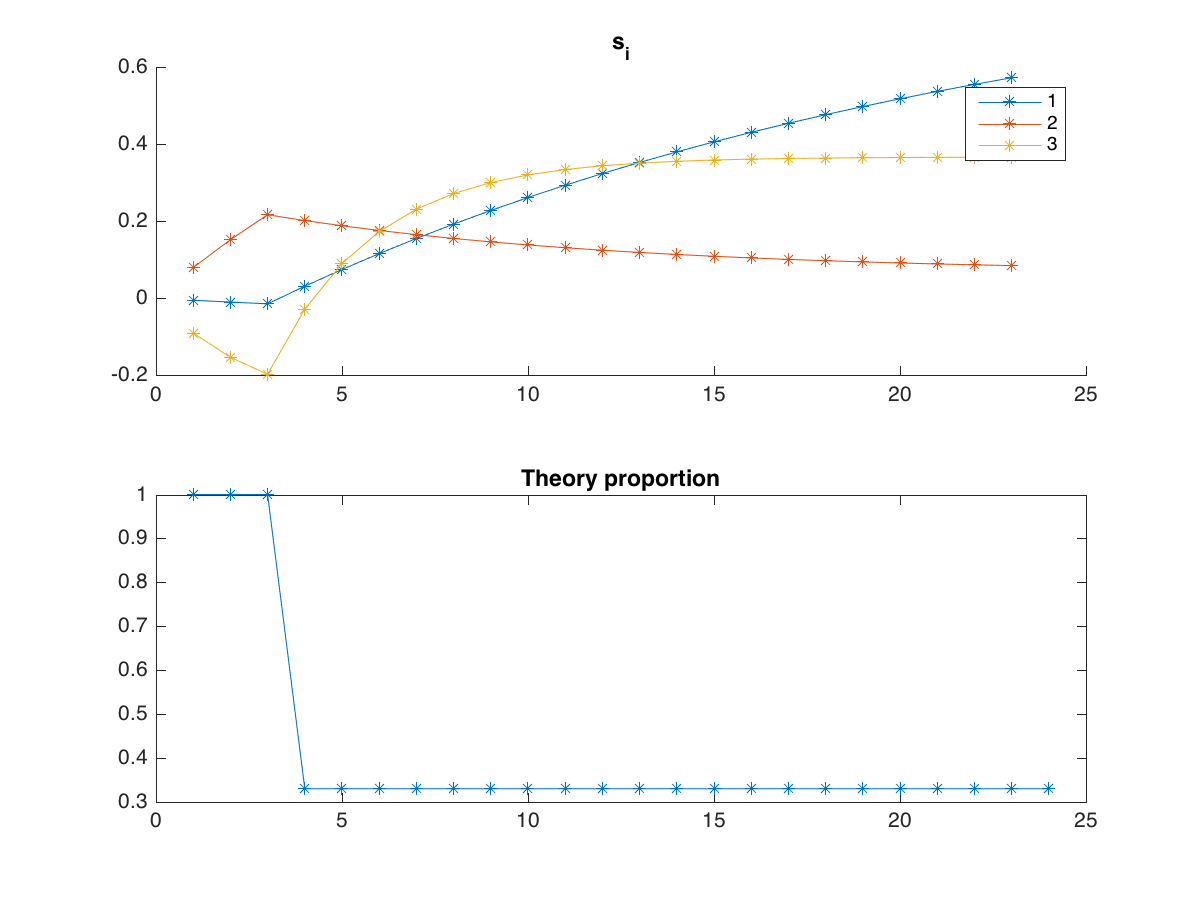
\includegraphics[width=.9\linewidth]{./img/plan1.png}
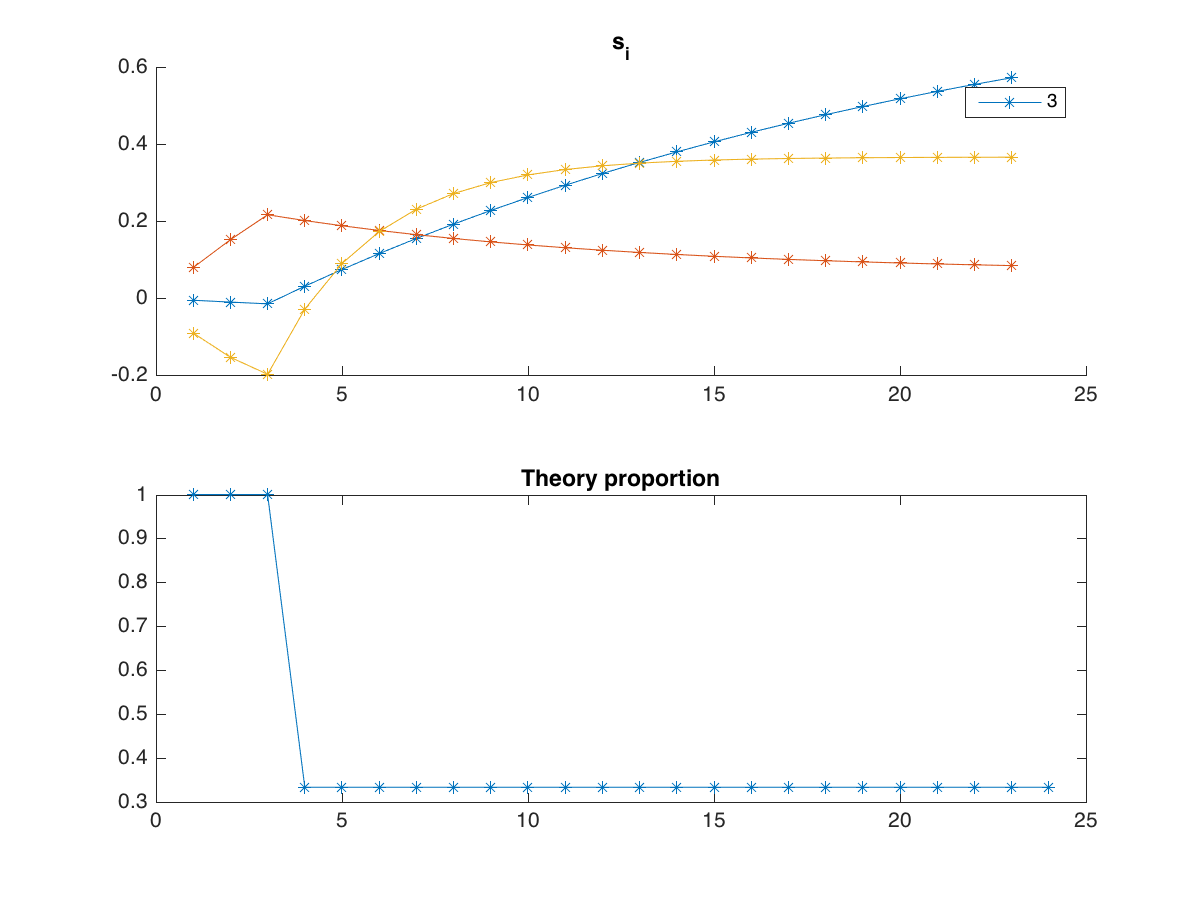
\includegraphics[width=.9\linewidth]{./img/plan2.png}
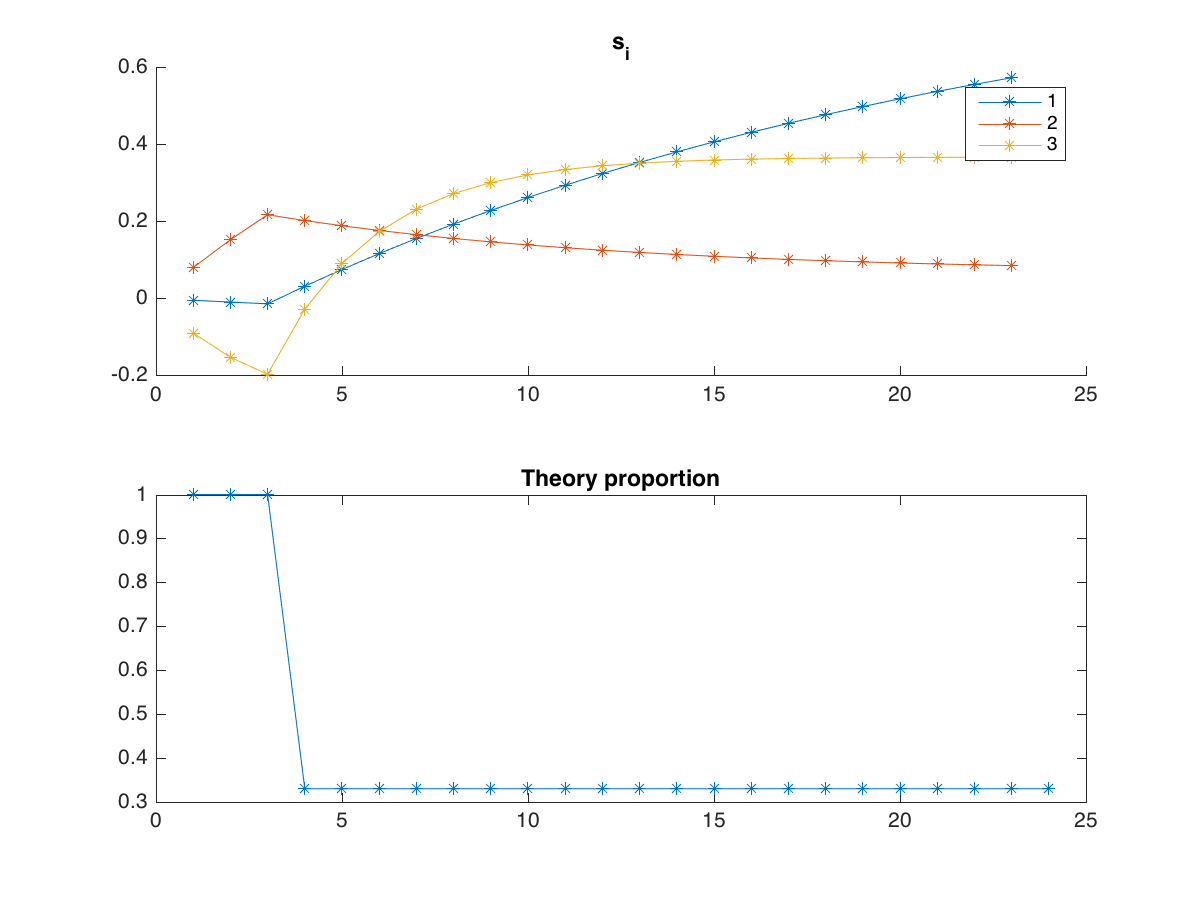
\includegraphics[width=.9\linewidth]{./img/plan3.png}


Optmizing the minimum off all three CES:
\begin{align}
  \text{maximize} \; & t \\
  \text{subject to} \; & A + T = 1,
  \\& A, T \ge 0
  \\& \sum_4^i A_j \le  2 \sum_4^i T_j \quad i = 4, \ldots, 24
  \\& t \le \langle \Theta^{(k)}, \alpha^{(k)} T + \beta^{(k)} A \rangle \quad k = 1,2,3
\end{align}



\begin{verbatim}
%% max min CES
cvx_begin 
variable T(num_periods)
variable t
maximize t
0 <= T <= 1
T(1:b) == 1
for i = 4 : num_periods
    sum(1 - T(b:i)) <= a* T(b:i)
end
for g = 1 : num_groups
    t <= ( Theta(g,:) * (alpha(g) * T + beta(g) * (1-T)) )
end
cvx_end

figures(4) = figure('visible', 'off')

subplot(2,1,1)
title('s_i')
% calculate s_i
for k=1:3
    s = zeros(num_periods+1, 1);
    for i=2:(num_periods+1)
        s(i) = (1- theta(k)) * s(i-1) + theta(k) * (alpha(k) * T(i-1) ...
                                                    + beta(k) * (1-T(i-1)));
    end
    table(4, k) = sum(s);

    hold on
    plot(s(2:num_periods), '*-')
end
subplot(2,1,2)
plot(T, '*-')
title('Theory proportion')

for p =1:4
    saveas(figures(p),[ 'plan' int2str(p)], 'png')
end

ans = table
\end{verbatim}



\begin{center}
\begin{tabular}{llll}
 & group 1 & group 2 & group 3\\
plan 1 &  &  & \\
plan 2 &  &  & \\
plan 3 &  &  & \\
plan 4 &  &  & \\
\end{tabular}
\end{center}


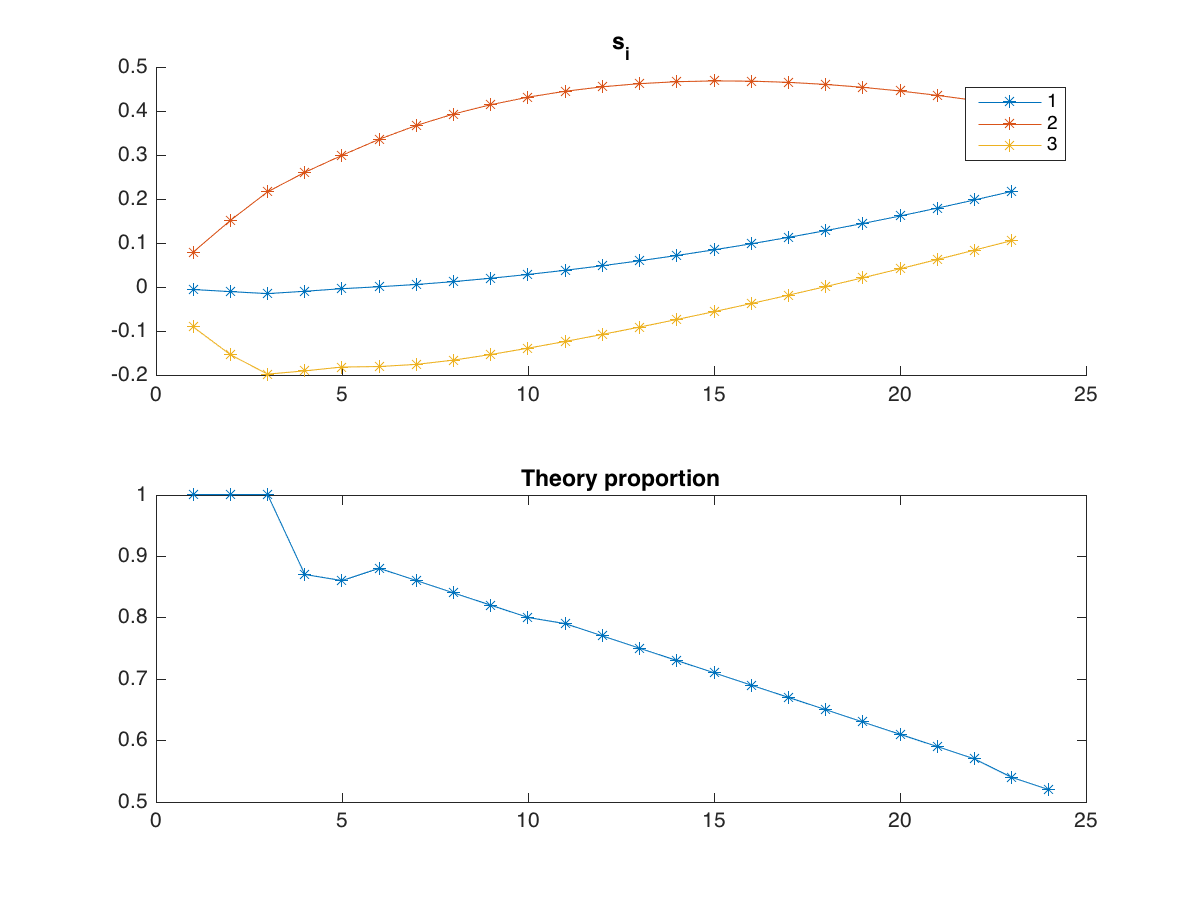
\includegraphics[width=.9\linewidth]{./img/plan4.png}


\section{Problem 3}
\label{sec:orgheadline3}
\(S \subseteq \mathbb R^n\)
Let \(C\) a convex contating set containing \(S\), and let \(x = \sum_i \lambda_i x_i\) convex combination of element of \(S\) and thus of element of \(C\), so \(x \in C\). Therefore \(conv(S) \subset \cap_{S \subset C, C \text{ convexe}} C\)

The convex hull is a convexe set containing \(S\), so \(\cap_{S \subset C, C \text{ convexe}} C \subset  conv(S)\).

c/c \(conv(S) = \cap_{S \subset C, C \text{ convexe}} C\).


\section{Problem 4}
\label{sec:orgheadline4}
a)
\(\mathcal G \rightarrow \mathcal G, Q \rightarrow Q_iQ\)  is an injection because \(Q_i\) is invertible, so it is a bijection (because \(\mathcal G\) is finite), therefore:
$$Q\bar x = \frac1k \sum_{Q \in \mathcal G} Q_iQ = \frac1k \sum_{Q \in \mathcal G} Qx = \bar x$$
so \(\bar x \in Q\).

b) \(f(\bar x) \le \sum_i \frac1k f(Q_ix) = \frac1k \sum_i  f(x) = f(x)\)

c) Let \(x\) be a solution to the convex \$\mathcal G\$-invariant. Then \(\bar x \in \mathcal F\) is also a solution. Indeed:
-- \$f\(_{\text{0}}\)(\bar x) \(\le\) f(\bar x) \$
-- for \(j\), \(f_j(x) \le 0 \implies \forall i f_j(Q_i x) \le 0 \implies  \frac1k \sum_i f_j(Q_i x) \le 0\)
-- \(f_j\) is convexe, so \(f_j(\bar x)  \le \frac1k \sum_i f_j(Q_i x) \le 0\)
c/c: \(f(\bar x) \le f(x)\) and \(\bar x\) is in the feasible set, which means \(\bar x\) is optimal.

d) Let \$\mathcal G \$ be the set of all permutations in \(\mathbb R^{n \times n}\). It is clear that this set is a finite (of size \(n!\) ) group.
Therefore we can adjoin the equality constraints \(Px = x \forall P \in \mathcal G\). Let \(x\) be apoint satisfying such condition, and let \(i, j \le n\), and \(Q\) be the matrix that permutates the ith and jth vector of the canonical basis. Then \(x_i = (Px)_i = x_j\). Therefore \(x\)  has the form \(x_11, x_1 \in \mathbb R\).

\section{Problem 5}
\label{sec:orgheadline5}

\#+name distance
\begin{verbatim}
1.9372
\end{verbatim}


1.9372

\section{Problem 6}
\label{sec:orgheadline6}

\begin{itemize}
\item \(P_1\) facet description
\(P_2\) vertex description
Algorithm: for each vertex \(v\) in \(P_2\) if \(v \in P_1\) (\(Av \le b\))

Complexity: \(O(D^2NM)\) where \(D\) is the dimension, \(M\) the number of facets, and \(N\) the number of vertices.

\item \(P_1\) vertex description \(y_1, \ldots, y_m\)
\(P_2\) vertex description \(x_1, \ldots, x_n\)
algorithm: Check if every vertex in \(P_2\) is a convex combination of the vertices of \(P_1\): \(y_1, \ldots, y_m\). For that, check if the following LP problems are feasible: for all vertex \(x\) in \(P_2\), \(\min_{\lambda} 0\) st \(\sum \lambda_i y_i = x, \sum_i \lambda_i = 1, \lambda > 0\)

\item \(P_1\) facet description \(A_1x \le b_1\)
\(P_2\) facet description \(A_2x \le b_2\)
algorithm: Check if every row  \(a_i^T\) in \(A_1\): Check that the following problem has a non negative solution:
\(\min_{A_2x \le b} (b_1)_i - a^T x\)
\end{itemize}
\end{document}
